\documentclass[xcolor=dvipsnames]{beamer}
\mode<presentation>
{
  \usetheme{Darmstadt}
%  \usetheme{Szeged}
  \usefonttheme{professionalfonts}
  \setbeamerfont*{frametitle}{size=\normalsize,series=\bfseries}
  \setbeamertemplate{navigation symbols}{}
  \definecolor{UVABlue}{RGB}{0,47,108}
  \definecolor{UVAOrange}{RGB}{229,114,0}
  \usecolortheme[named=UVABlue]{structure}

  \setbeamercolor*{palette secondary}{use=structure,fg=white,bg=UVABlue}
%  \setbeamercolor*{palette tertiary}{use=structure,fg=white,bg=UVABlue}
  \setbeamercolor*{block title}{use=structure,fg=white,bg=UVABlue}
  \setbeamercolor*{block title example}{use=structure,fg=white,bg=UVAOrange}
  \setbeamercolor*{block body example}{use=structure,bg=white}
  }
\usepackage{amsmath} \usepackage{amssymb} \usepackage{amsfonts}
\usepackage{amsthm} \usepackage{enumerate} \usepackage[all]{xy}
\usepackage{ulem}
\usepackage{tikz-cd}
\usepackage[absolute,overlay]{textpos}
\usetikzlibrary{decorations.markings,arrows}
\setlength{\TPHorizModule}{1mm}
\setlength{\TPVertModule}{1mm}

\beamertemplateballitem

\mode<presentation>
{
  \usetheme{Warsaw}
%\usecolortheme[named=OliveGreen]{structure}
  \setbeamercovered{transparent}
}

\usepackage[english]{babel}
\usepackage[latin1]{inputenc}
\usepackage{times}
\usepackage[T1]{fontenc}

\setbeamercovered{invisible}


\def\souta{\bgroup \ULdepth=-.7ex \ULset}


\newcommand{\proj}{\ensuremath{\mathrm{proj}}}
\newcommand{\D}{\ensuremath{\mathcal{D}}}
\newcommand{\Z}{\mathbb{Z}}
\newcommand{\R}{\mathbb{R}}
\newcommand{\C}{\mathbb{C}}
\newcommand{\sC}{\mathcal{C}}
\newcommand{\Q}{\mathbb{Q}}
\newcommand{\E}{\mathbb{E}}
\renewcommand{\S}{\mathbb{S}}
\newcommand{\cA}{\mathcal{A}}
\newcommand{\cM}{\mathcal{M}}
\newcommand{\cE}{\mathcal{E}}
\newcommand{\cp}{\mathcal{p}}
\newcommand{\otfr}{\otimes_{F(R)}}
\newcommand{\otr}{\otimes_R}
\newcommand{\KK}{\mathbb{K}}
\newcommand{\kk}{\mathbbm{k}}
\newcommand{\otzg}{\otimes_{\Z[G]}}
\newcommand{\ot}{\otimes}
\newcommand{\bphi}{\bar{\phi}}
\newcommand{\bpsi}{\bar{\psi}}
\newcommand{\FF}{\mathbb{F}}
\newcommand{\LL}{\mathbb{L}}
\newcommand{\Cay}{\mathrm{Cay}}
\newcommand{\CAT}{\mathrm{CAT}}
\newcommand{\geom}{\mathrm{geom}}
\newcommand{\rhob}{\bar{\rho}}
\newcommand{\inte}{\mathrm{int}}
\newcommand{\cS}{\mathcal{S}}
\newcommand{\cG}{\mathcal{G}}
\newcommand{\Stab}{\mathrm{Stab}}
\newcommand{\SL}{\mathrm{SL}}
\newcommand{\FP}{\mathrm{FP}}
\newcommand{\normal}{\trianglelefteq}
\newcommand{\bZ}{\bar{Z}}
\newcommand{\st}{\ensuremath{\mathrm{st}}}
\newcommand{\lk}{\ensuremath{\mathrm{lk}}}


\newtheorem{ques}{Question}
\newtheorem{Theo}{Theorem}
\newtheorem{prop}{Proposition}
\newtheorem{cor}[Theo]{Corollary}
\newtheorem{Conj}[Theo]{Conjecture}
\newtheorem{lem}[Theo]{Lemma}
\newtheorem{assume}[Theo]{Assumptions}
\theoremstyle{definition}
\newtheorem{defn}[Theo]{Definition}
\newtheorem{Exam}[Theo]{Example}



\def\adots{\mathinner{\mkern2mu\raise0pt\hbox{.}  % antidiagonal dots
\mkern2mu\raise4pt\hbox{.}\mkern1mu
\raise7pt\vbox{\kern7pt\hbox{.}}\mkern1mu}}

\title[RGD Systems with Exceptional Links]{Finite Generation of RGD systems with Exceptional Links}
\author{Mark Schrecengost}
\institute{Department of Mathematics\\University of Virginia}

\date{April 23, 2020}

\subject{Talks}


\begin{document}


\begin{frame}
  \titlepage
\end{frame}

\begin{frame}{Coxeter Systems}
	\begin{defn}
		A Coxeter System is a pair $(W,S),$ consisting of a group $W$ and a set $S\subset W$ such that $W$ is generated by $S,$ and $W$ admits a presentation of the form
		\[
			W=\langle s|s\in S,\;s^2=1,\;(st)^{m(s,t)}=1\text{ for all }s,t\in S\rangle
		\]
		where $m(s,t)\in \mathbb{N}\cup\{\infty\}.$
	\end{defn}
	\pause
	Common examples include:
	\begin{enumerate}
		\item $S_n$
		\item $D_{2n}$
		\item Reflection groups
	\end{enumerate}
\end{frame}

\begin{frame}{Coxeter Systems}
Some basic facts about Coxeter Systems:
\begin{itemize}
	\pause
\item For every $J\subset S$ we can form a subgroup $W_J=\langle s\in J\rangle$
	\pause
\item The subgroups $W_J$ are all distinct, and the set $J$ can be recovered as $J=W_J\cap S$
	\pause
\item We will call $W_J$ standard subgroups, and cosets of the form $wW_J$ standard cosets
	\pause
\item The length function $\ell$ on $W$ has nice properties, and there is an algorithm to write any element of $w$ as a minimal length word.
\end{itemize}
\end{frame}

\begin{frame}{The Coxeter Complex}
	\begin{defn}[Coxeter Complex]
		For each Coxeter system $(W,S),$ there is a simplicial complex $\Sigma=\Sigma(W,S),$ where the simplices of $\Sigma$ correspond to standard cosets of $W,$ and the face relation is given by reverse inclusion.
	\end{defn}
	\begin{itemize}
		\pause
	\item The maximal simplices, called \emph{chambers}, of $\Sigma$ are all the same dimension, and correspond to the elements of $W.$
			\pause
		\item Each simplex has a type given by $\tau(wW_J)=S\setminus J,$ and a cotype $J.$
			\pause
		\item A \emph{panel} is a co-dimension 1 simplex, which will have cotype $s$ for some $s\in S.$ We say that two chambers are $s$-adjacent if they share a common $s$ panel. Two chambers are adjacent if they are $s$-adjacent for some $s\in S.$
	\end{itemize}
\end{frame}

\begin{frame}{The Coxeter Complex}
	Some useful facts and definitions about the Coxeter Complex
\begin{enumerate}
	\pause
\item $W$ acts on $\Sigma$ by left multiplication, and acts simply transitively on Chambers
	\pause
\item We call $C=\{1\}=W_{\emptyset}$ the fundamental chamber
	\pause
\item A gallery is a sequence of chambers $D_0,\dots,D_n$ such that $D_i$ and $D_{i+1}$ are adjacent for all $i.$
	\pause
\item We can define a metric $d$ on the chambers $\mathcal{C}(\Sigma)$ where $d(D,E)$ is the length of the shortest gallery from $D$ to $E.$
\end{enumerate}
\end{frame}

\begin{frame}{Examples}
	\begin{textblock}{100}(0,15)
		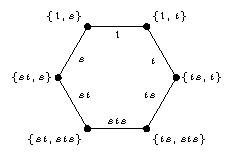
\includegraphics[width=2 in]{diagrams/hexagon.pdf}
	\end{textblock}
	\begin{textblock}{100}(50,15)
	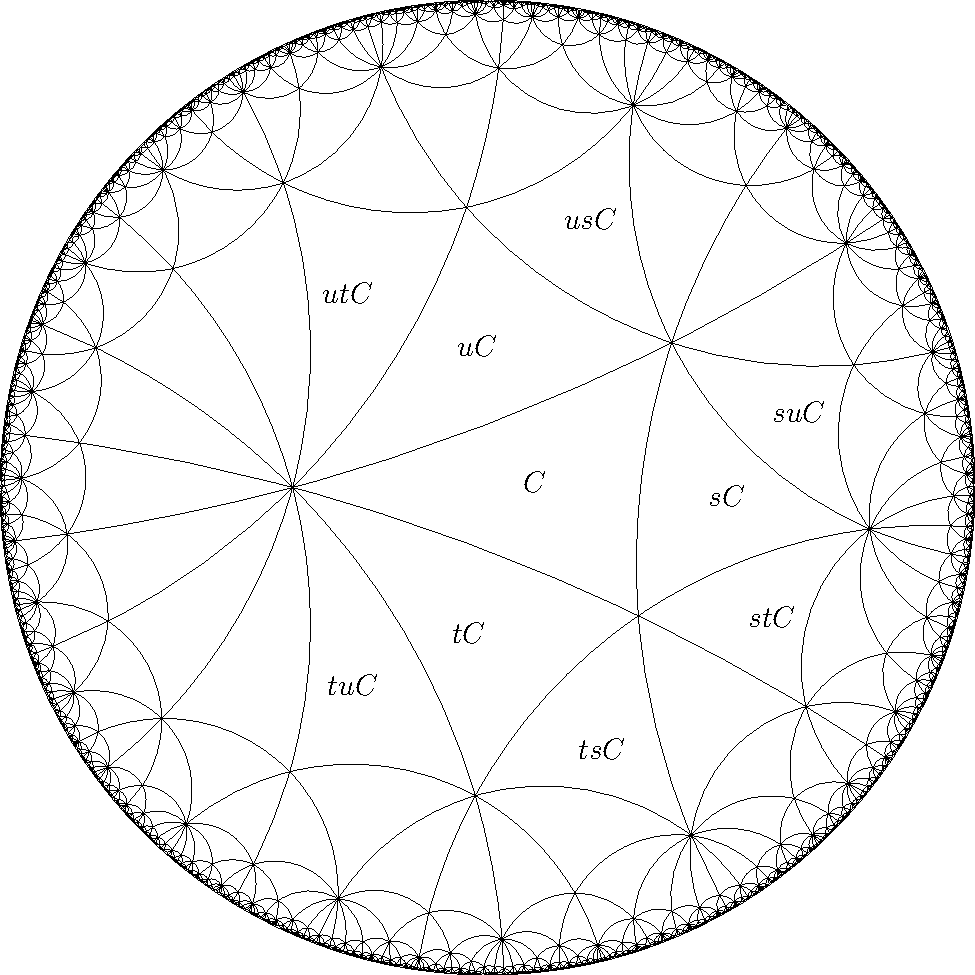
\includegraphics[width=70 mm]{diagrams/hyp.pdf}
	\end{textblock}
	\begin{textblock}{100}(10,55)
	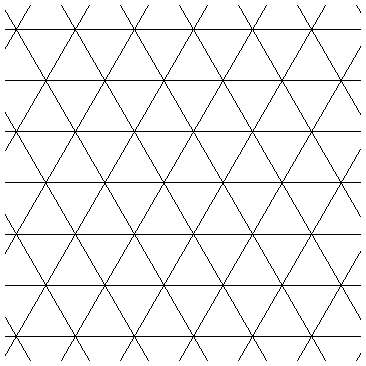
\includegraphics[width=1.33 in]{diagrams/affinetriangle.pdf}
	\end{textblock}
\end{frame}

\begin{frame}{Links and Stars}
	\begin{defn}[Links and Stars]
		If $A$ is a simplex of $\Sigma$ then the star of $A,$ denoted $\st(A),$ is the set of all chambers containing $A.$ The link of $A,$ denoted $\lk(A),$ is all the faces of the chamber of $\st(A)$ which are disjoint from $A.$
	\end{defn}
	\bigskip
	\pause
	If $A$ is a simplex of cotype $J$ then $\lk(A)$ is canonically isomorphic to $\Sigma(W_J,J).$ \\
\end{frame}

\begin{frame}{Links and Stars}
	\begin{center}
	\includegraphics<1>[height=0.9\textheight]{diagrams/link1.pdf}%
	\includegraphics<2>[height=0.9\textheight]{diagrams/link3.pdf}%
	\includegraphics<3>[height=0.9\textheight]{diagrams/link2.pdf}%
	\end{center}
\end{frame}

\begin{frame}{Projections and Roots}
\begin{defn}[Projections]
	If $A$ is a simplex of $\Sigma,$ and $D$ is a chamber of $\Sigma$ then there is a unique chamber $E$ in $\st(A)$ such that $d(D,E')=d(D,E)+d(E,E')$ for all $E'\in \st(A).$ The chamber $E$ is called the projection of $D$ onto $A$ and is denoted $\proj_A(D).$
\end{defn}
\pause
We want to think about Coxeter groups as Reflection groups, and roots give us the half spaces that any reflection should define.
\pause
\begin{defn}[Roots]
	If $D$ and $D'$ are adjacent chambers of $\Sigma,$ then the set of chambers $\alpha=\{E\in \Sigma|d(D,E)<d(D',E)\}$ is called a root of $\Sigma.$ The boundary of a root is called a wall, and is denoted $\partial \alpha.$ We say a root is positive if it contains the fundamental chamber $C.$
\end{defn}
\end{frame}

\begin{frame}{Links, Projections, and Roots}
All of these objects interact nicely with each other:
\begin{itemize}
	\pause
	\item The action of $W$ also acts on the set of links, projections and roots.
		\pause
	\item A root through $A$ is positive if and only if it contains the projection of $C$ onto $A.$
		\pause
	\item The roots of $\lk(A)$ are given by intersections of roots with $A\in \partial \alpha.$ We will call these the roots through $A.$
\end{itemize}
\end{frame}

\begin{frame}{Links, Projections, and Roots}
\begin{center}
	\includegraphics<1>[height=0.9\textheight]{diagrams/root1.pdf}
	\includegraphics<2>[height=0.9\textheight]{diagrams/root2.pdf}
\end{center}\end{frame}

\begin{frame}{Buildings}
\begin{defn}[Building]
	A building $\Delta$ is a simplical complex which is a union of a family of sub-complexes $\mathcal{A},$ called apartments, such that
	\begin{enumerate}
		\item[(B0)] Each $\Sigma\in \mathcal{A}$ is a Coxeter Complex
		\item[(B1)] Any two simplices are contained in a common apartment
		\item[(B2)] For any two apartments, there is an isomorphism between them which fixes the intersection
	\end{enumerate}
\end{defn}
\pause
Buildings were introduced by Tits to study groups of Lie type.\\
\smallskip
When working in buildings, we have many of the same definitions as in Coxeter complexes, and in most cases it will suffice to work in suitable choices of apartments instead of the entire building. 
\end{frame}

\begin{frame}{Groups Acting on Buildings}
	Groups acting on buildings in certain ways yield nice algebraic properties
	\begin{itemize}
		\pause
		\item Strongly transitive actions give BN-Pairs
			\pause
		\item A stronger condition called Moufang gives RGD systems, which means that $G$ is generated by some family of groups $U_\alpha$ for all the roots of $\Delta,$ and another group $T.$
			\pause
		\item Most common examples are groups of Lie type and Kac-Moody groups over fields. Specific examples include $\mathrm{SL}_n(k)$ and $\mathrm{SL}_n(k[t,t^{-1}]).$
	\end{itemize}
	\pause
	The axioms of an RGD system are quite strong, and they imply certain commutator relations $[U_\alpha,U_\beta]$ for pairs of roots.\\
\end{frame}

\begin{frame}{Presentation of $U_+$}
	If $(G,(U_\alpha)_{\alpha\in \Phi},T)$ is an RGD system of type $(W,S),$ then we have a root group $U_\alpha$ for every root of the Coxeter complex $\Sigma(W,S).$\\
	\pause
	\bigskip
	The subgroup $U_+=\langle U_\alpha|\alpha\in \Phi_+\rangle$ has a nice presentation where the only relations are those in the root groups $U_\alpha,$ and commutator relations between pre-nilpotent pairs of roots. As long as $W$ is infinite, this presentation is in terms of infinitely many generators, but we still have the following question
	\pause
	\begin{ques}
		When is $U_+$ finitely generated?		
	\end{ques}
\end{frame}

\begin{frame}{Finite Generation of $U_+$}
	\begin{Theo}[Abramenko, Van Maldeghem]
		If $\Delta$ satisfies (co) then $U_+$ is generated $\{U_{\alpha_s}\}$ where $\alpha_s$ is the root separating $C$ and $sC.$
\end{Theo}
\bigskip
\pause
As a Corollary, $U_+$ is finitely generated if all root groups are finitely generated, in particular, if they are finite.\\
\bigskip
\pause
\begin{defn}[Condition (co)]
A building satisfies (co) if the set of chambers opposite a given chamber is gallery connected.
\end{defn}
\end{frame}

\begin{frame}{Condition (co)}
A building will satisfy condition (co) if all of its co-dimension 2 links satisfy (co).
\bigskip
\pause
\begin{Theo}
	Every rank 2 Moufang building satisfies (co) except the following finite (twisted) Chevalley groups
	\[
		C_2(2)\quad G_2(2)\quad G_2(3) \quad {}^2F_4(2)
	\]
\end{Theo}
\pause
\bigskip
We want to look at buildings and RGD systems where one of the co-dimension 2 links are one of the 4 exceptional cases.
\end{frame}

\begin{frame}{Assumptions}
	\begin{assume}
		Assume that $(G,(U_\alpha)_{\alpha\in \Phi},T)$ is an RGD system of type $(W,S)$ with associated building $\Delta.$ Additionally assume
		\begin{equation}
	\label{assume}
	\tag{A} 
\begin{aligned}
	&S=\{s,t,u\},\: a=m(s,t),b=m(s,u),c=m(t,u)\\
	&3\le a,b,c<\infty\\
	&U_\alpha \text{ is finitely generated for all }\alpha\in \Phi\\
	&[U_\alpha,U_\beta]=1\text{ when }\alpha,\beta \text{ are nested}
\end{aligned}
\end{equation}
and also assume that $\Delta$ has a vertex of type $s$ with an exceptional link.
	\end{assume}
\end{frame}

\begin{frame}{Heuristic for the Proof}
\begin{enumerate}
	\item Each vertex $v$ has a set of positive roots $\alpha_1,\dots,\alpha_n$ which pass through $v,$ and subgroups $U_v=\langle U_i\rangle$ and $U'_v=\langle U_1,U_n\rangle.$
		\pause 
	\item If $v$ is exceptional then $U_v\neq U'_v$ and there is a surjective homomorphism $\phi_v:U_v\to H$ where $H$ is a non-trivial cyclic group. This homomorphism sends $U'_v$ to the identity.
		\pause
	\item We can sometimes extend this homomorphism to a map $\tilde{\phi}_v:U_+\to H$ so that $\tilde{\phi}_v(U_\beta)=\{1\}$ for all other roots $\beta.$
		\pause
	\item Since $\tilde{\phi}_v$ is still surjective, at least 1 root passing through $v$ must be in any generating set of $U_+.$
\end{enumerate}
\end{frame}

\begin{frame}{General Case}
	\begin{Theo}[S.]
		If $(G,(U_\alpha)_{\alpha\in \Phi},T)$ is an RGD system satisfying $\eqref{assume},$ with an exceptional link, then $U_+$ is not finitely generated if at least 2 of $a,b,c$ is greater than or equal to 4.	
\end{Theo}
\begin{Theo}[S.]
	If $(G,(U_\alpha)_{\alpha\in \Phi},T)$ is an RGD system satisfying $\eqref{assume},$ where $a=b=3,$ and $\Delta$ has a vertex with link associated to $G_2(2)$ then $U_+$ is not finitely generated.
\end{Theo}
These results cover all but 3 cases.
\end{frame}

\begin{frame}{Proof Sketch}
	\begin{itemize}
		\item Fix a chamber $C$ and an apartment $\Sigma$ containing $C.$ There will be a vertex $x$ of $C$ with an exceptional link and a non-trivial homomorphism $\phi_x:U_x\to H.$
			\pause
		\item Extend this map to $\tilde{\phi}_x:U_+\to H$ by sending all other roots to the identity.
			\pause
		\item Check that this map is well defined
	\end{itemize}
	\pause
	What do the relations in $U_+$ look like?
	\begin{enumerate}
		\pause
	\item Relations in $U_\alpha$
		\pause 
	\item Nested root groups commute, so that $[U_\alpha,U_\beta]=1$
		\pause
	\item $[U_\alpha,U_\beta]\subset U_{(\alpha,\beta)}$ for non-nested pre-nilpotent pairs
	\end{enumerate}
\end{frame}

\begin{frame}{Proof Sketch (cont.)}
	\begin{columns}[c]
\begin{column}{0.42\textwidth}
	We need to check that the right side of every commutator relation of the third type is sent to the identity.\\[.2 in]
\pause
It is enough to check that the non-simple roots at $x$ are simple everywhere else.
\end{column}
\begin{column}{0.58\textwidth}
	\only<1-2>{\color{white}\rule{\textwidth}{\textwidth}}%
	\only<3>{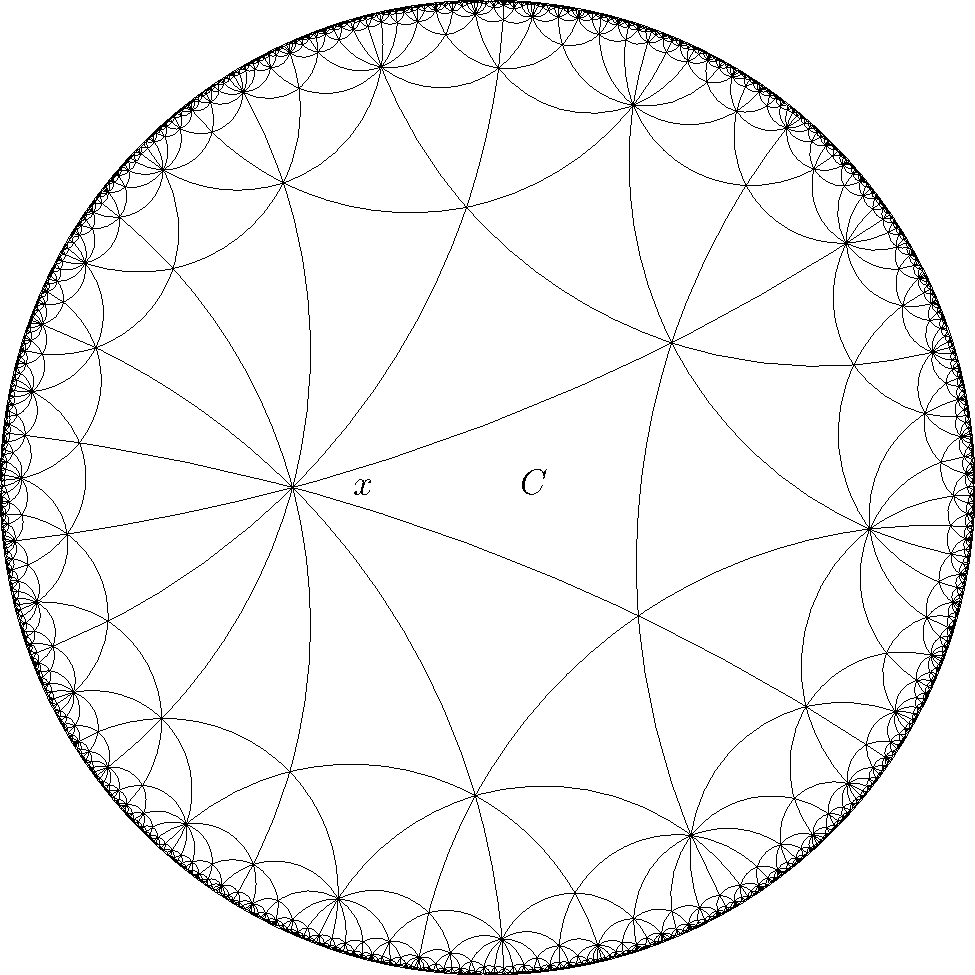
\includegraphics[width=\textwidth]{diagrams/simple1.pdf}}%
	\only<4>{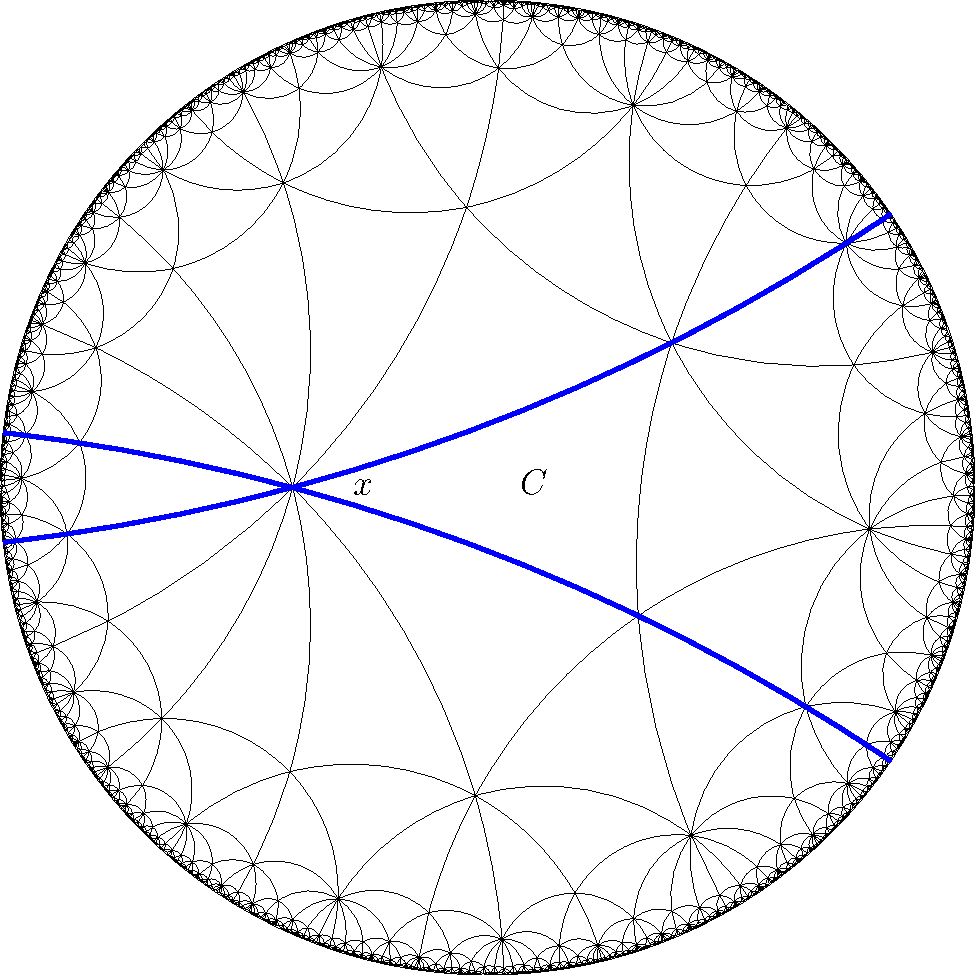
\includegraphics[width=\textwidth]{diagrams/simple2.pdf}}%
	\only<5>{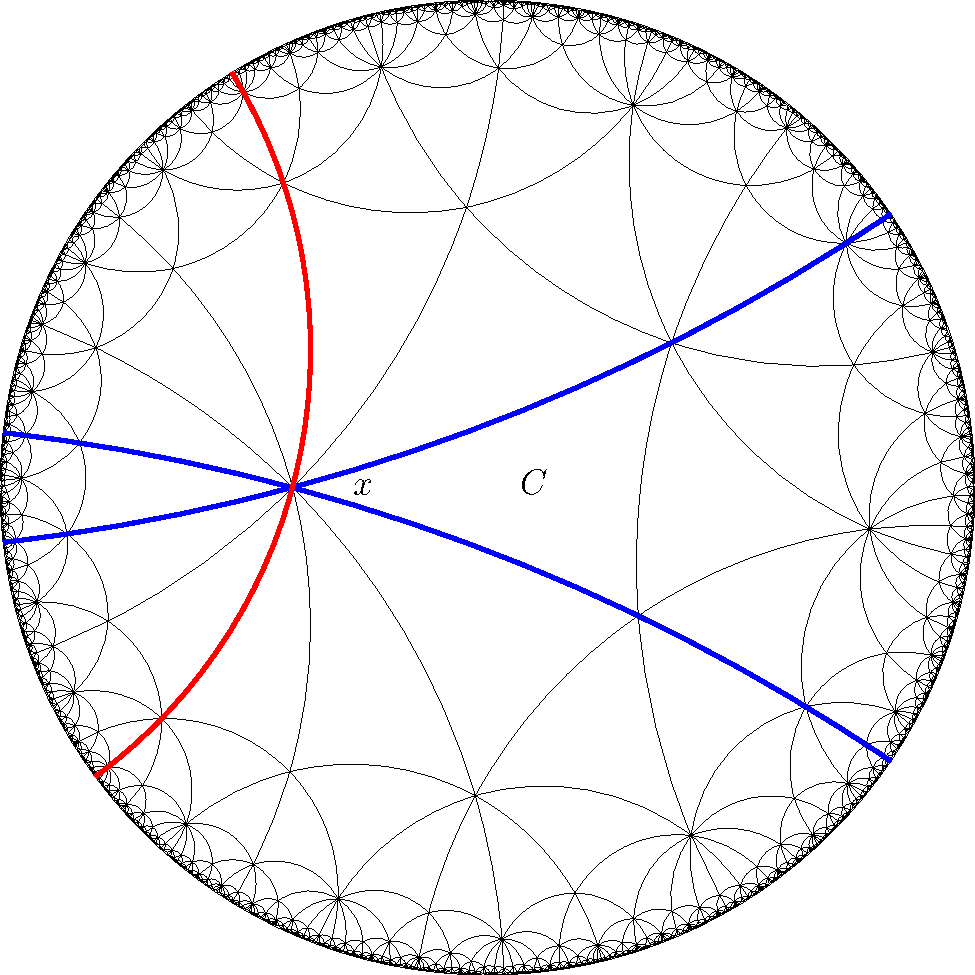
\includegraphics[width=\textwidth]{diagrams/simple3.pdf}}%
	\only<6>{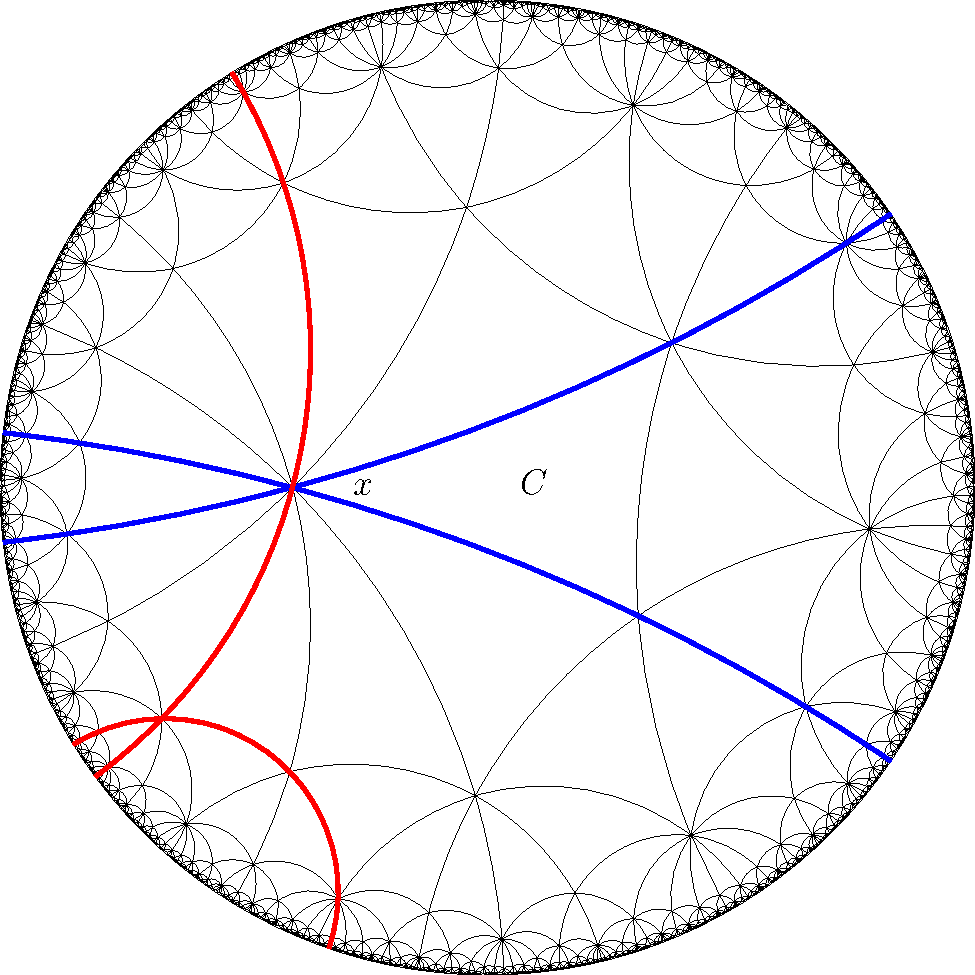
\includegraphics[width=\textwidth]{diagrams/simple4.pdf}}%
	\only<7>{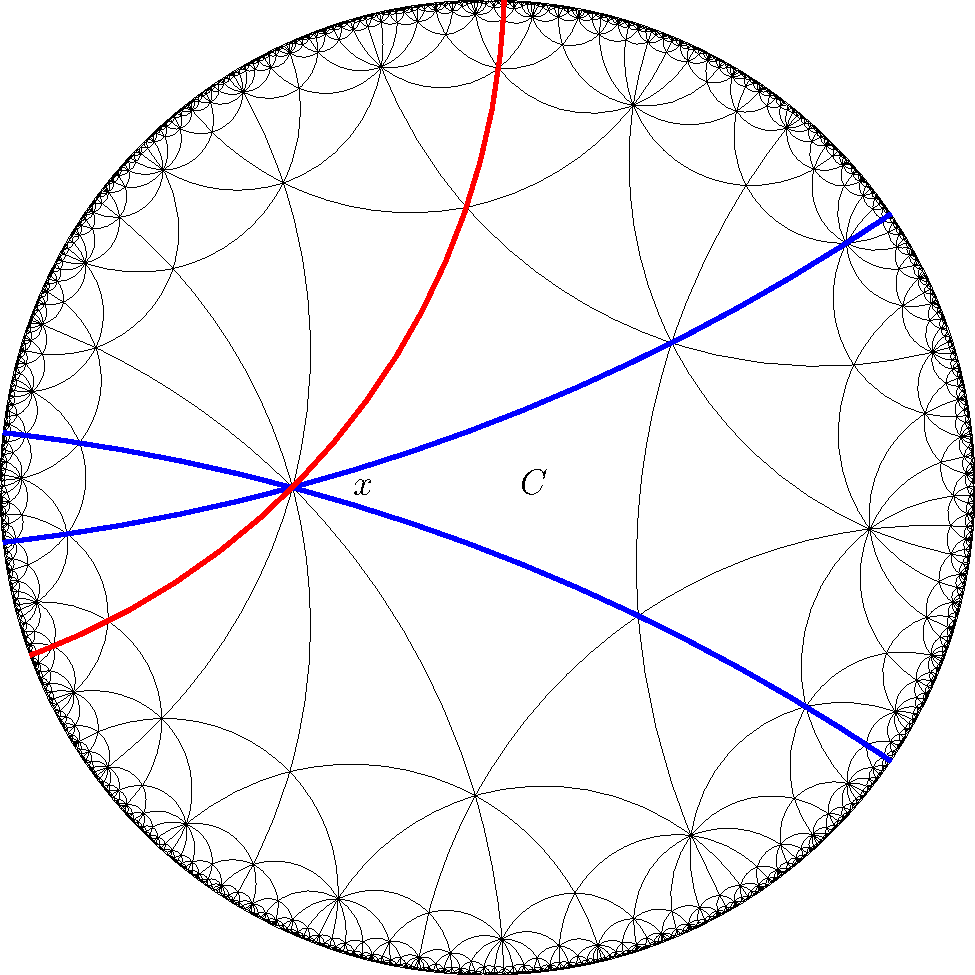
\includegraphics[width=\textwidth]{diagrams/simple5.pdf}}%
	\only<8>{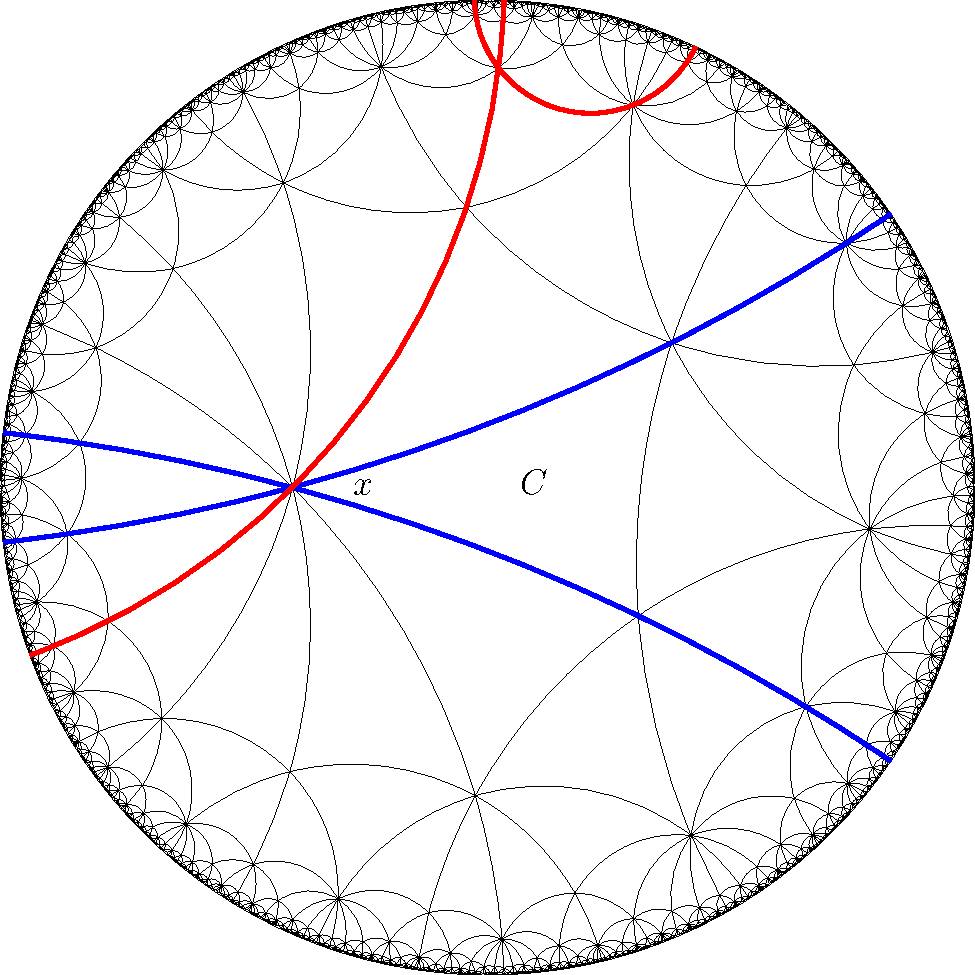
\includegraphics[width=\textwidth]{diagrams/simple6.pdf}}%
	\only<9>{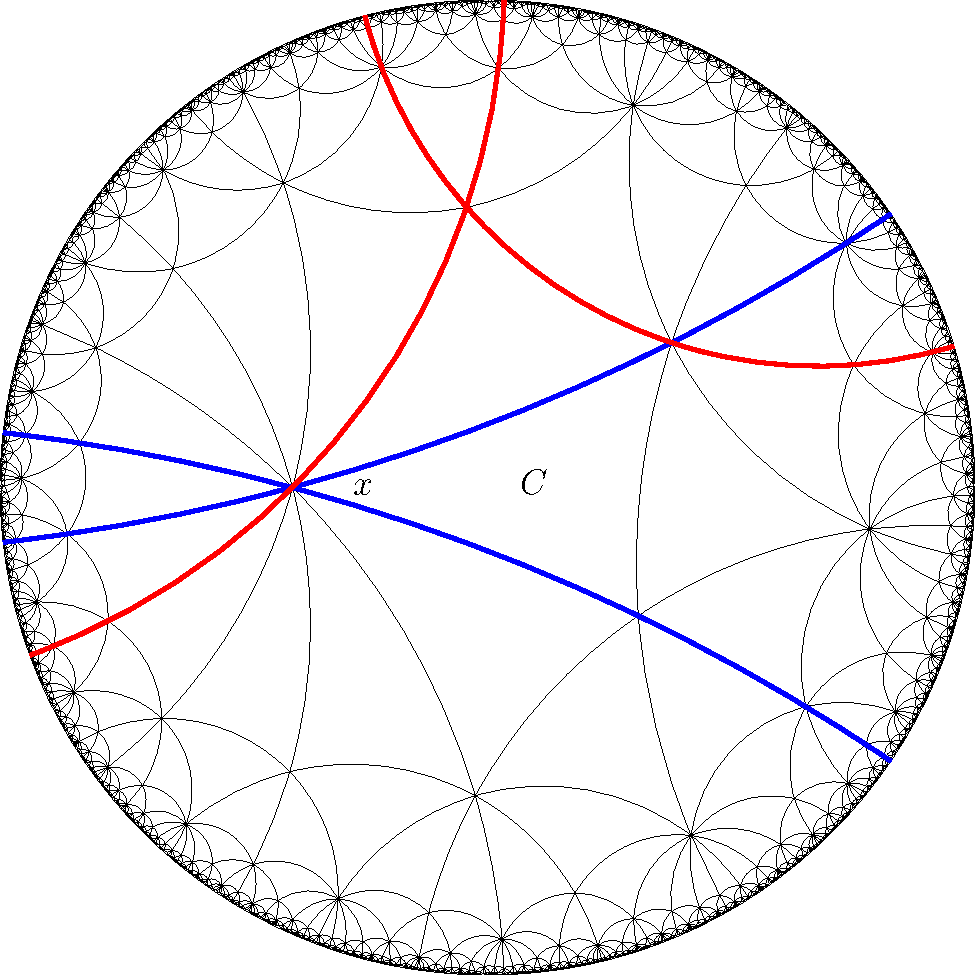
\includegraphics[width=\textwidth]{diagrams/simple7.pdf}}%
	\only<10>{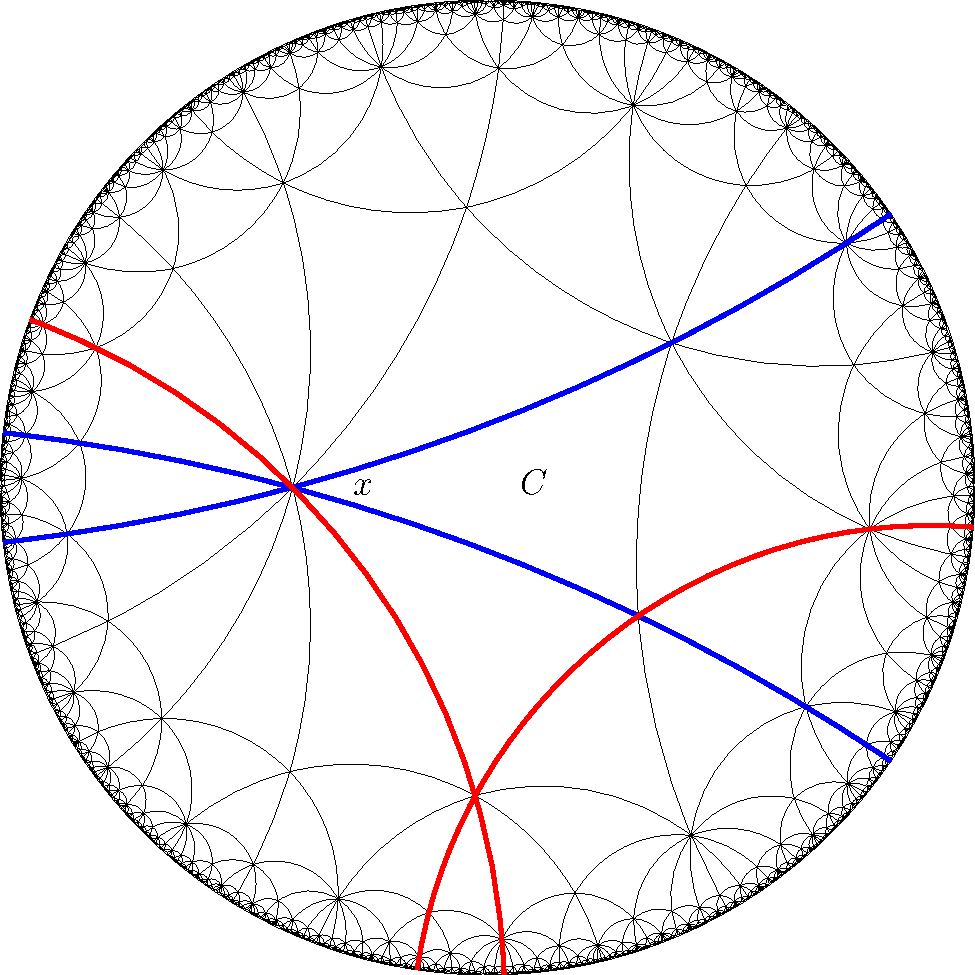
\includegraphics[width=\textwidth]{diagrams/simple8.pdf}}%
	\only<11>{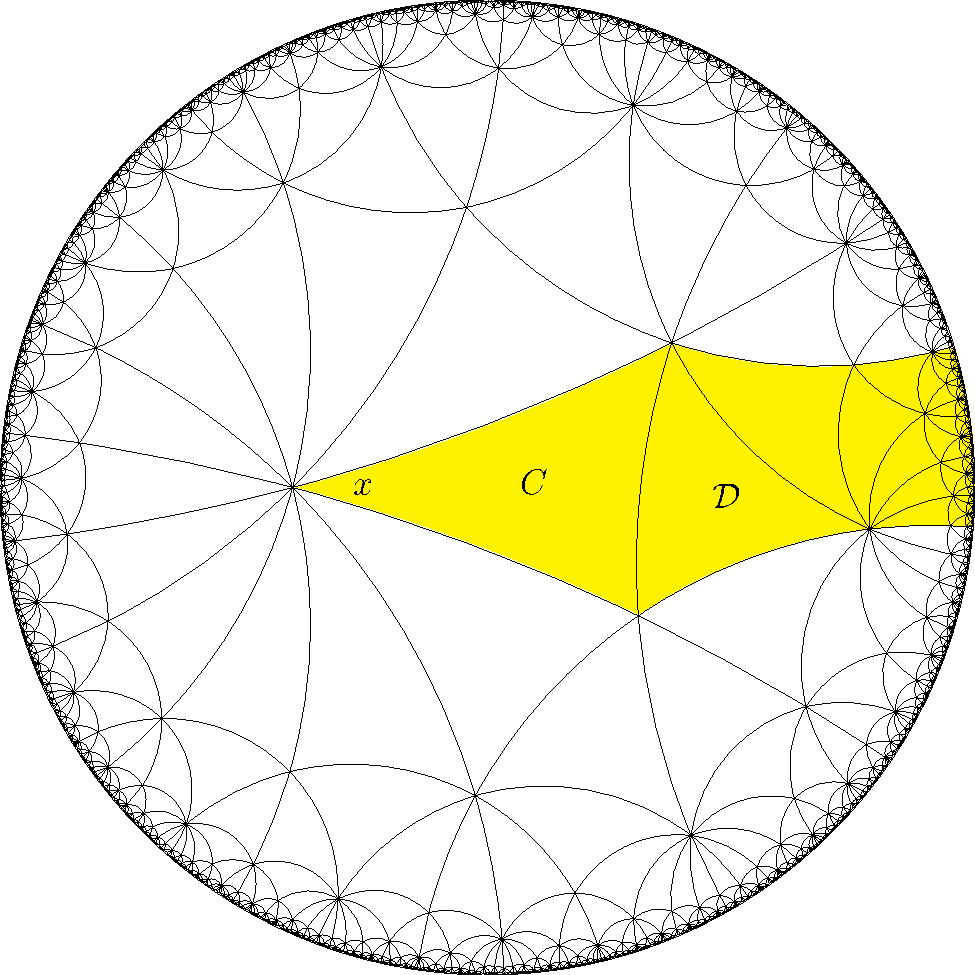
\includegraphics[width=\textwidth]{diagrams/simple9.pdf}}%
\end{column}
\end{columns}
\end{frame}

\begin{frame}{Proof Sketch (cont.)}
	\begin{itemize}
	\item The simple root condition shows that $\tilde{\phi}_x$ would exist if $C$ lies anywhere in $\mathcal{D}.$
		\pause
	\item Apply the action of $W$ with appropriate group elements to get a family of $\tilde{\phi}_v$ for chambers of $\mathcal{D}.$
		\pause
	\item Check these maps are distinct, and the vertices $v$ do not lie on finitely many walls.
	\end{itemize}
	\pause
	The last two steps can be checked by switching back to the group theory of $W.$ We have candidates $(sut)^kx,$ and these last two properties can be phrased in terms of length conditions.\\
	\pause
	\bigskip
	For example, to check that $(sut)^kx$ lies in $\D,$ one thing we must check is that $\ell((sut)^k)\le \ell(t(sut)^k)$ which we can do by finding a reduced decomposition.

\end{frame}

\begin{frame}{The Region $\D$}
	\begin{itemize}
		\item When two of $a,b,c$ are at least 4, this region $\D$ has infinitely many chambers, and we can prove $U_+$ is not finitely generated.
		\pause
	\item When $a=b=3,$ then the region $\D$ is finite, and this approach must be modified.
		\pause
	\item If the exceptional vertex has link associated to $G_2(2)$ then we can relax the condition on simple roots, and enlarge $\D$ to get another region which is still infinite.
	\end{itemize}
	\pause
	\bigskip
	What about the remaining cases?
\end{frame}
\begin{frame}{Finitely Generated Cases}
	\begin{Theo}[S.]
		If $(G,(U_\alpha)_{\alpha\in \Phi},T)$ is an RGD system satisfying \eqref{assume} such that $a=b=3,$ and the vertex of type $s$ has link associated to $C_2(2)$ or $G_2(3),$ then $U_+$ is finitely generated.
	\end{Theo}
	Note: The case with ${}^2F_4(2)$ is impossible.
\end{frame}

\begin{frame}{Sketch of Proof}
	\begin{itemize}
		\item Define $d(\alpha,C)$ to be the minimal distance to a chamber which borders $\partial \alpha.$
		\pause
	\item Define subgroups $U_n$ generated by all roots within a certain distance from $C.$
		\pause
	\item Each $U_n$ is finitely generated, and their union is $U_+.$
		\pause
	\item When we hit vertices with exceptional links, we can ``go the other way around''
	\end{itemize}
\end{frame}

\begin{frame}{Sketch of Proof}
	\begin{center}
		\includegraphics<1>[height=0.85\textheight]{diagrams/3341.pdf}%
		\includegraphics<2>[height=0.85\textheight]{diagrams/3342.pdf}%
		\includegraphics<3>[height=0.85\textheight]{diagrams/3343.pdf}%
		\includegraphics<4>[height=0.85\textheight]{diagrams/3344.pdf}%
		\includegraphics<5>[height=0.85\textheight]{diagrams/3345.pdf}%
		\includegraphics<6>[height=0.85\textheight]{diagrams/3346.pdf}%
		\includegraphics<7>[height=0.85\textheight]{diagrams/3347.pdf}%
	\end{center}
\end{frame}

\begin{frame}{Sketch of Proof (cont.)}
	\begin{itemize}
		\item For every chamber $D\neq C,$ there is a vertex $v$ so that $D\neq \proj_v(C).$
		\pause
	\item Inductively, this shows that $U_k=U_+$ for large enough $k,$ and in fact $U_+=U_2.$
		\pause
	\end{itemize}
	\bigskip
	This technique also yields another proof of the result when $\Delta$ satisfies (co).\\
	\bigskip
	\pause
	This generating set of $U_2$ is not minimal, and there are generating sets (consisting of root groups) with 5 roots, compared to 3 roots when condition (co) is satisfied.
\end{frame}

\begin{frame}{Questions?}
\begin{center}
	\Large
	Thank you.\\
\bigskip
\bigskip
Any Questions?

\end{center}
\end{frame}


\end{document}
